\begin{titlepage}
\newgeometry{top=2cm,bottom=1cm,left=3cm}
\definecolor{capri}{rgb}{0.0, 0.75, 1.0}
%left colorfill

\begin{tikzpicture}[remember picture, overlay]
  \node [anchor=north west, inner sep=0pt]
    at (current page.north west)
    {
      \begin{tikzpicture}[every node/.append style = {anchor=center}]
        \begin{scope}
          \fill[black!100]   ( 120:1) rectangle (20mm, 310mm);
        \end{scope}
      \end{tikzpicture}
    };
\end{tikzpicture}

\begin{tabular}[\textwidth]{b{9.5cm}c} %adjust the length (currently 8cm) to move the department name at appropriate position. It must be towards the right edge as shown in the template

   
\includegraphics[width=30mm, height=30mm]{1200px-IIT_Madras_Logo.png}  & \shortstack[l]{DEPARTMENT OF \\ ELECTRICAL ENGINEERING \\ INDIAN INSTITUTE OF \\ TECHNOLOGY \\ MADRAS \\ CHENNAI-600 036} \\
   
\end{tabular}

\vspace{-0.4cm}

\hspace{-0.75cm} \rule{19cm}{1mm}

\vspace{0.5cm}
\hspace{0.8cm} %adjust this to put the title in the center of the page
\begin{tabular}{c}
     {\normalfont\selectfont{\LARGE \textbf{AN IMPROVED SLIDING MODE CONTROL}}} \\[0.5cm]
     {\normalfont\selectfont{\LARGE \textbf{SCHEME FOR POWER QUALITY}}} \\[0.5cm]
     {\normalfont\selectfont{\LARGE \textbf{CONDITIONERS IN DISTRIBUTION SYSTEM}}} \\[0.5cm]
     {\normalfont\selectfont{\LARGE \textbf{}}} \\[0.5cm]
\end{tabular}
%
\vspace{2cm} %b/w title and graphic
\hspace{3cm} %using manual spacing instead of "center" tag, to bring text in the center of white part.
\begin{tabular}{c}
     %\vspace{1cm}
     %\fbox{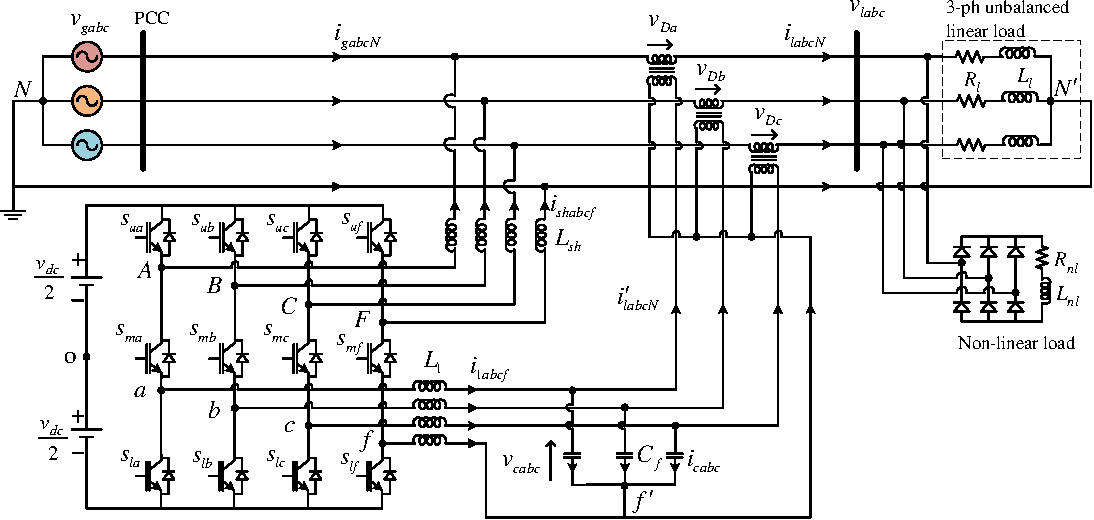
\includegraphics[width=50mm, height=50mm]{figures/Chapter_6/Mine/4leg_UPQC_L.pdf}}\\
     \fbox{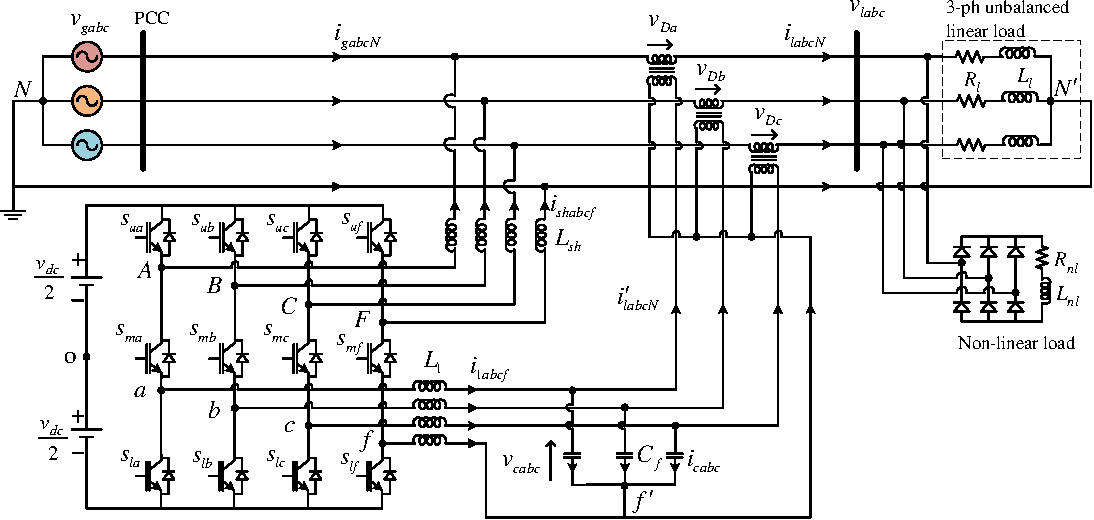
\includegraphics[scale=0.5]{figures/Chapter_6/Mine/4leg_UPQC_L.pdf}}\\
%    
	 \\  
     \vspace{-0.5cm}
     \textit{A thesis}\\[0.45cm]
     \vspace{-0.5cm}
     \textit{Submitted by}\\[0.45cm]
     \vspace{-0.5cm}
     \textbf{LOKESH N}\\ \\ \\[0.45cm]
%     
     \vspace{-0.25cm}
     \textit{For the award of the degree}\\[0.45cm]
     \vspace{-0.25cm}
     \textit{Of}\\[0.45cm]
     \vspace{-0.25cm}
     \textbf{DOCTOR OF PHILOSOPHY}\\[0.85cm]
     JANUARY, 2024
%
\vspace{-0.5cm}
\end{tabular}\\[0.45cm]
%
\textcircled{c} 2024 Indian Institute of Technology Madras
%
\end{titlepage}